\chapter{Conversione AD e convertitori - parte I}

\begin{figure}[h]
    \centering
    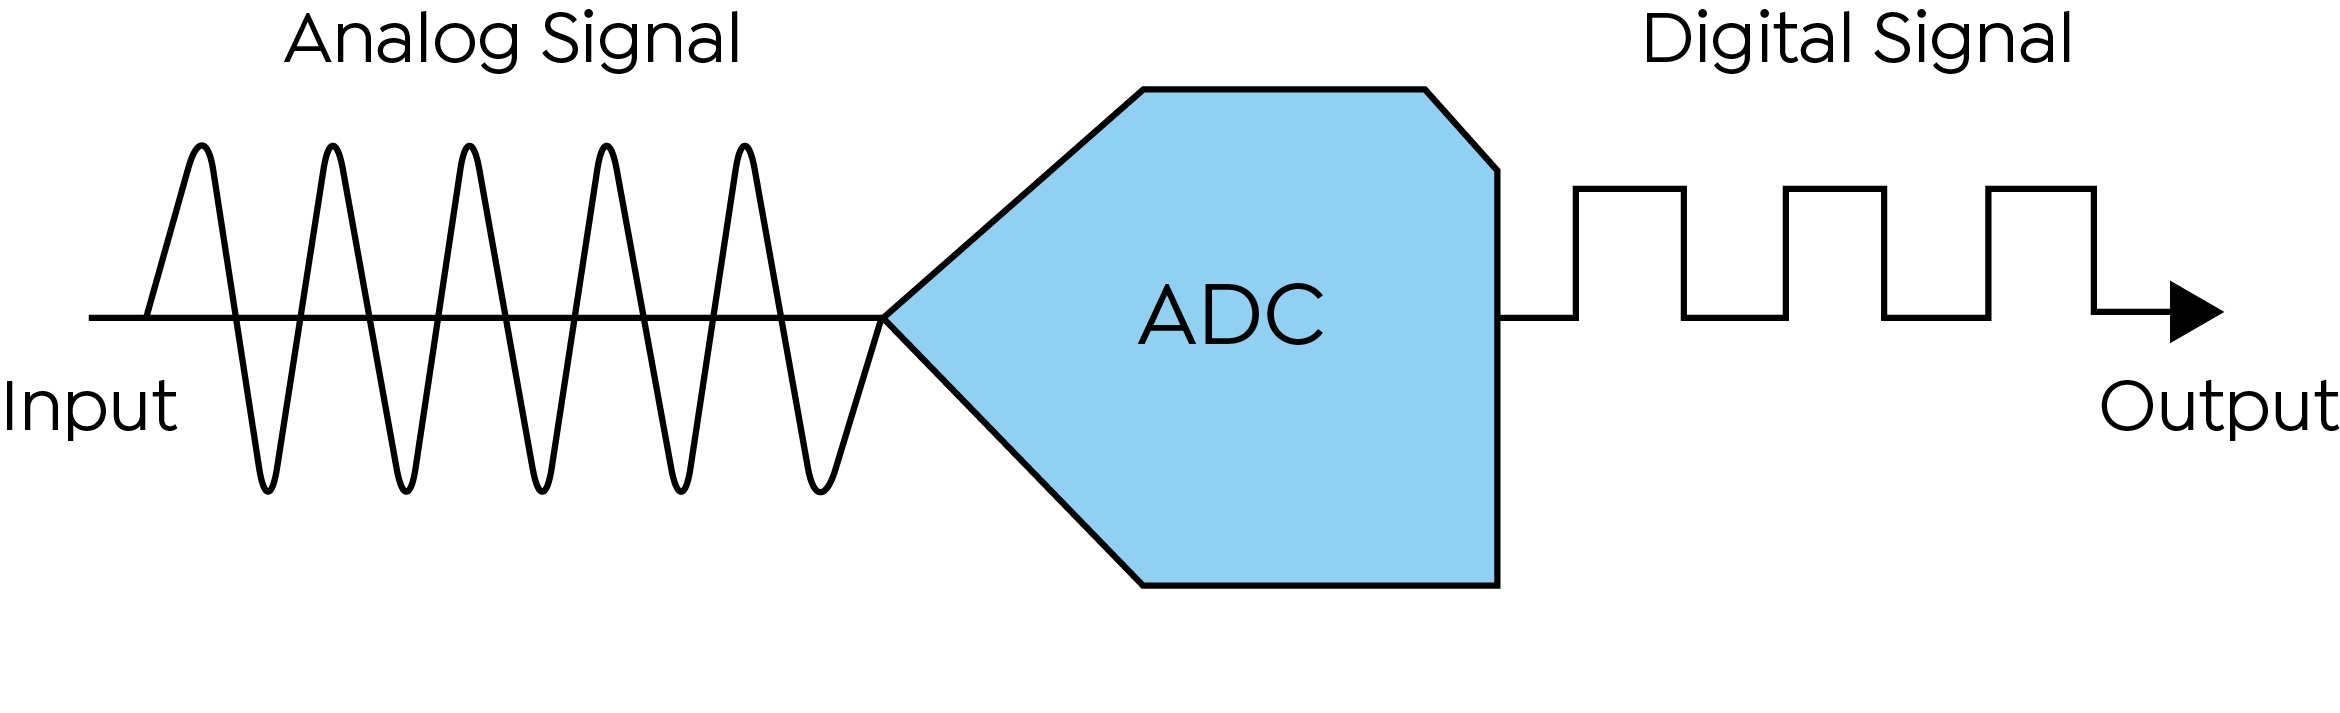
\includegraphics[scale = 0.3]{EBV_ST-Analog_Blockdiagramm_EBVA022-Figure3.jpg}
\end{figure}

\newpage 

\begin{tcolorbox}
    I concetti dei capitoli riguardo la conversione AD e dei vari convertitori sono già stati approfonditi in precedenti materie di questo corso di laurea. \newline 
    Adesso verranno approfonditi in ambito misuristico    
\end{tcolorbox}

\section{Segnali analogici e digitali}
\footnote{Slide della prof | SDME 3.Conversione AD e Convertitori - Parte I | pag 3 - 4 \\  
Appunti | 2025-03-18 | pag 2 - 3}

Si definisce segnale analogico un segnale che può essere rappresentato mediante una funzione del tempo che gode di due proprietà: 

\begin{itemize}
    \item la funzione è definita per ogni valore del tempo 
    \item la funzione è continua
\end{itemize}

Grazie a queste due proprietà, un segnale analogico ha infiniti valori. \newline 

Un esempio di segnale analogico: 

\begin{figure}[h]
    \centering
    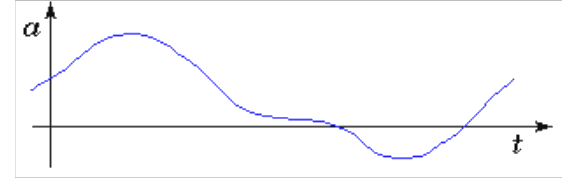
\includegraphics[scale = 0.4]{Esempio segnale analogico.png}
\end{figure}

Da un punto di notazione matematica, possiamo definire un segnale analogico come: 

{
    \Large 
    \begin{equation}
        \begin{cases}
            a = f(t) 
            \\ 
            t \in \mathbb{R}
            \\ 
            a \in \mathbb{R}
        \end{cases}
    \end{equation}
} 

Dagli infiniti valori dei casi continui, passiamo ai finiti valori 
(discreti valori) dei segnali digitali. \newline 

Un segnale digitale è rappresentato da una funzione a tempo discreto e quantizzata. \newline 

Ciò significa che: 

\begin{itemize}
    \item la funzione è definita solamente in un insieme numerabile di istanti, tipicamente equi-spaziata 
    \item la funzione è dotata di codominio costituito da un insieme discreto e numerabile di valori
\end{itemize}

La quantizzazione potrebbe avvenire con "quanti" di ampiezza diversa. \newline 

Un esempio di segnale digitale: 

\begin{figure}[h]
    \centering
    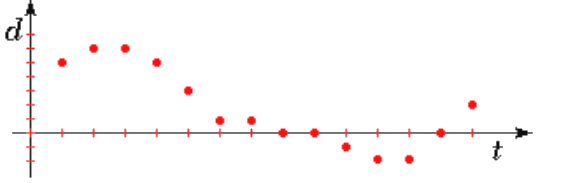
\includegraphics[scale = 0.4]{Esempio di segnale digitale.png}
\end{figure}

La funzione passa da un livello "consentito" ad un altro senza poter attraversare tutti i valori intermedi, 
quindi, da un punto di vista grafico, la funzione non è definita tra due punti. \newline 

La distanza tra due punti, nell'asse delle ascisse del tempo t, viene definito come periodo di campionamento $T_c$. \newline 

Da un punto di notazione matematica, possiamo definire un segnale digitale come: 

{
    \Large 
    \begin{equation}
        \begin{cases}
        d = f[n T_c]
        \\
        n \in \mathbb{Z}  
        \\ 
        d \in \mathbb{Z}
        \end{cases}
    \end{equation}
}

\begin{tcolorbox}
    Per distinguere tra segnale analogico e discreto, 
    come nel corso di DSP di Stefano Squartini, userò la notazione tra parentesi tonde () per indicare un segnale analogico, 
    mentre a parentesi quadre [ ] per un segnale discreto 
\end{tcolorbox}


\newpage 

\section{Interesse alle misure elettroniche}
\footnote{Slide della prof | SDME 3.Conversione AD e Convertitori - Parte I | pag 5 \\  
Appunti | 2025-03-18 | pag 3}

Tra tutte le tipologie di segnali, c'è interesse rispetto ai segnali elettrici analogici perchè presentano le seguenti proprietà: 

\begin{itemize}
    \item amplificabilità diretta 
    \item trasmissibilità a distanza 
    \item registrabilità 
    \item elaborabilità (come scritto precedentemente, si utilizzano gli OpAmp per svolgere i calcoli matematici)
\end{itemize}

Dai segnali analogici a quelli digitali, la misura diventerà una sequenza di numeri. \newline 

I segnali elettrici numerici, o digitali, esaltano ulteriormente queste proprietà: 

\begin{itemize}
    \item trasmissibilità a distanza (beneficia della natura discreta della f nel tempo) 
    \item registrabilità (segnali numerici consentono una maggiore densità di registrazione)
    \item elaborabilità (mediante algoritmi eseguiti da microprocessori o DSP)
    \item reiezione ai disturbi (un segnale digitale non risiede di disturbi fino ad una certa entità)
\end{itemize}

La possibilità di impiegare algoritmi eseguiti da microprocessori o DSP permette di elaborare il segnale con nuove versioni del 
software senza costruire fisicamente un nuovo circuito. \newline 

\newpage 

\subsection{Analogico vs Digitale: occupazione della linea}
\footnote{Slide della prof | SDME 3.Conversione AD e Convertitori - Parte I | pag 6 - 7 \\  
Appunti | 2025-03-18 | pag 3}


Dal punto di vista dell'occupazione della linea, il segnale analogico occupa permanentemente la linea di trasmissione, 
mentre quello digitale ne permette la condivisione con altri segnali. \newline 

Considerando due segnali analogici di un cavo jack stereo: 

\begin{figure}[h]
    \centering
    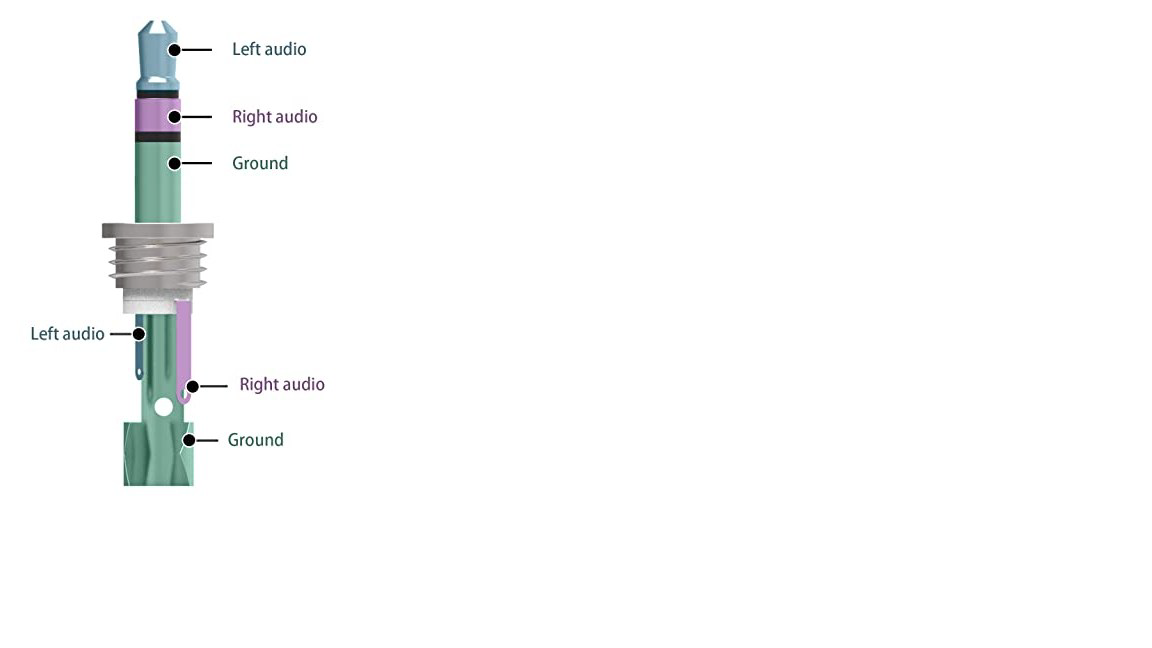
\includegraphics[scale = 0.4]{cavo jack stereo.png}
\end{figure}

Essendo un segnale definito in ogni istante, 
ogni segnale analogico necessita della linea in ogni singolo istante di tempo in cui esso esiste.\newline 

Quindi per trasmettere due segnali analogici, come in figura: 

\begin{figure}[h]
    \centering
    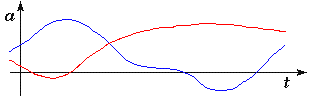
\includegraphics[scale = 1]{Due segnali analogici.png}
\end{figure}

occorrono 3 linee, due per i segnali e una per la massa come in figura: 

\begin{figure}[h]
    \centering
    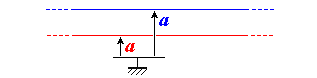
\includegraphics[scale = 1]{Due linee e massa in comune.png}
\end{figure}

Il segnale digitale necessita della linea solo nei singoli istanti di tempo in cui esso esiste ed è definito come si vede in figura: 

\begin{figure}[h]
    \centering
    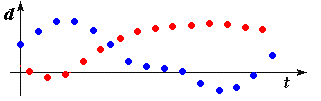
\includegraphics[scale = 0.8]{Due segnali digitali .png}
\end{figure}

\newpage 

Negli altri istanti, si può lasciare la linea libera e consentire la trasmissione di altri segnali digitali, come in figura: 

\begin{figure}[h]
    \centering
    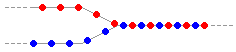
\includegraphics[scale = 0.8]{Condivisione nella stessa linea.png}
\end{figure}


Per inviare più segnali nella stessa linea, 
si possono multipare i segnali o in altri canali o in frequenza, 
e poi demultiplarli in ricezione, come si è studiato nel corso di Telecomunicazioni Digitali con Franco Chiaraluce. \newline 


\subsection{Analogico vs Digitale: registrabilità}
\footnote{Slide della prof | SDME 3.Conversione AD e Convertitori - Parte I | pag 8 \\  
Appunti | 2025-03-18 | pag 4}

Anche la registrabilità di un segnale digitale è migliore di quella di un segnale analogico. \newline 

Il segnale digitale è registrabile in maniera più "fedele e compatta" di quello analogico. \newline 

Il segnale analogico viene conservato in supporti magnetici, che con il tempo perdono la loro stabilità e fedeltà. \newline 

Invece, il segnale digitale è generalmente più stabile e può essere copiato in più dispositivi molto più facilmente 
dei dispositivi analogici. \newline 

\subsection{Analogico vs Digitale: elaborabilità}
\footnote{Slide della prof | SDME 3.Conversione AD e Convertitori - Parte I | pag 9 \\  
Appunti | 2025-03-18 | pag 4 }

Il segnale digitale è elaborabile in maniera più "potente" di quello analogico. \newline 

Il segnale analogico può essere elaborato mediante amplificatori operazioni, i quali sono circondati da una rete circuitale 
come nella seguente figura: 

\begin{figure}[h]
    \centering
    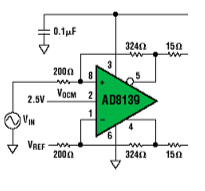
\includegraphics[scale = 0.8]{Esempio di OpAmp con rete circuitale.png}
\end{figure}

Al contrario, il segnale digitale può essere elaborato con un microprocessore o un DSP (Digital Signal Processor), 
cioè un dispositivo dedicato alla elaborazione numerica. \newline 

\subsection{Analogico vs Digitale: reiezione ai disturbi}
\footnote{Slide della prof | SDME 3.Conversione AD e Convertitori - Parte I | pag 10 \\  
Appunti | 2025-03-18 | pag 4}

Il segnale digitale ha una maggiore reiezione ai disturbi di quello analogico perchè 
il valore analogico ha infiniti valori, invece il segnale digitali ha valori finiti e "consentiti". \newline 

\newpage 

\section{Conversione analogico - digitale}
\footnote{Slide della prof | SDME 3.Conversione AD e Convertitori - Parte I | pag 11 \\  
Appunti | 2025-03-18 | pag 4}

La conversione AD (in inglese ADC: Analog to Digital Conversion) si attua con tre fasi in successione: 

\begin{enumerate}
    \item Campionamento 
    \item Quantizzazione 
    \item Codifica
\end{enumerate}

Il campionamento, partendo da un segnale analogico come il seguente: 

\begin{figure}[h]
    \centering
    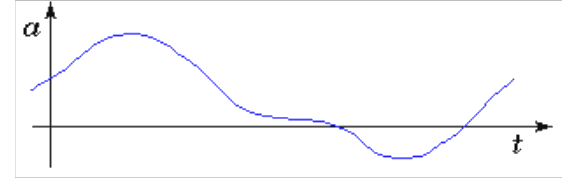
\includegraphics[scale = 0.6]{Esempio segnale analogico.png}
\end{figure}

si può applicare il campionamento. \newline 

Il campionamento attua la discretizzazione dell'asse dei tempi e si definiscono gli istanti di campionamento equi-spaziati tra loro, quindi non si ha una perdita di informazione. \newline 

Il segnale campionato, da quello analogico, diventerà: 

\begin{figure}[h]
    \centering
    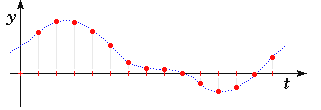
\includegraphics[scale = 1]{Segnale analogico campionato.png}
\end{figure}


Una volta che il segnale è stato campionato, lo si quantizza. \newline 

Per quantizzazione si intende la discretizzazione delle ampiezze, quindi una perdita di informazione. \newline 

Il segnale quantizzato diventerà: 

\begin{figure}[h]
    \centering
    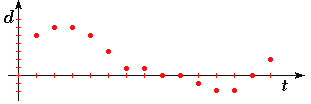
\includegraphics[scale = 1]{Segnale quantizzato.png}
\end{figure}

Una volta quantizzato, il segnale viene codificato. \newline 

Per codifica si intende che viene assegnato a ciascun livello di quantizzazione una parola di codice, 
usualmente binaria, univocamente determinata. \newline 

Il segnale codificato diventerà: 

\begin{figure}[h]
    \centering
    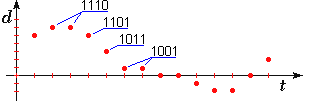
\includegraphics[scale = 1]{Segnale codificato.png}
\end{figure}

\newpage 

Dal punto di vista misuristico, le fasi più interessanti sono le prime due: campionamento e quantizzazione. \newline 

\newpage 

\section{Teorema fondamentale del campionamento}
\footnote{Slide della prof | SDME 3.Conversione AD e Convertitori - Parte I | pag 12 \\  
Appunti | 2025-03-18 | pag 4 -5}

Per il campionamento, è stato rivoluzionario il teorema del campionamento scritto dal matematico 
Claude. \newline 

Di seguito il teorema fondamentale del campionamento: 

\begin{figure}[h]
    \centering
    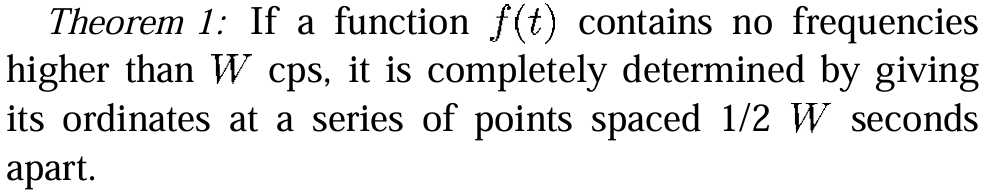
\includegraphics[scale = 0.5]{Teorema fondamentale del campionamento originale.PNG}
\end{figure}

\begin{tcolorbox}
    Shannon pubblicò il suo teorema nella seguente rivista: 
    "Claude E. Shannon Communication in the Presence of Noise
Proceedings of the IRE, vol. 37, no. 1, pp. 10-21, Jan. 1949" 
consultabile al seguente link \\ \url{https://webusers.imj-prg.fr/~antoine.chambert-loir/enseignement/2020-21/shannon/shannon1949.pdf}
\end{tcolorbox}

Visto che il teorema è stato pubblicato nel 1949, alcune terminologie sono diverse da quello al giorno d'oggi. \newline 

Le seguenti terminologie sono: 

\begin{itemize}
    \item cps è un'abbreviazione di cycles per second, nei giorni odierni utilizziamo l'indicazione di Hz 
    \item per ordinates si intendono i valori istantanei 
\end{itemize}

La traduzione italiana, con i seguenti adattamenti, del teorema fondamentale del campionamento è la seguente: \newline 

Se la funzione f(t) contiene nessuna frequenza maggiore di W Hz, è completamente determinata dai 
suoi valori istantanei spaziati da una serie di punti spaziati di $\frac{1}{2W}$ secondi tra di loro. \newline 

Questo teorema ci dice che, se gli istanti di campionamento sono opportunamente individuati, 
la funzione che si ottiene andando a prelevare il valore istantaneo del segnale solo in quegli istanti è completamente determinata, quindi non si ha perdita di informazione. \newline 

\newpage 

\section{La Delta di Dirac e il campionamento}
\footnote{Slide della prof | SDME 3.Conversione AD e Convertitori - Parte I | pag 13 - 14 \\  
Appunti | 2025-03-18 | pag 5}

Il teorema di Shannon fa riferimento ai valori istantanei (le ordinate) della funzione, 
prelevati in corrispondenza degli istanti di campionamento. \newline 

Per prelevare un segnale in un singolo istante, matematicamente, si ricorre alla funzione Delta di Dirac. \newline 

Se bisogna svolgere il campionamento in tutti gli istanti della funzione, bisogna applicare la seguente formula:

{
    \Large 
    \begin{equation}
        g_s (t) = g(nT) \cdot \sum_{n = - \infty}^{+ \infty} \delta (t - nT)
    \end{equation}
}

ovvero, un "treno" di Delta di Dirac, cioè una Delta di Dirac shiftata al valore nT della funzione. \newline 

\begin{tcolorbox}
    Il tema lo ho già approfondito nei miei appunti di Teoria dei segnali nel capitolo 
    1.3 Delta di Dirac \\\url{https://github.com/ciccio25/appunti-teoria-dei-segnali/blob/main/Appunti%20Teoria%20dei%20segnali.pdf} .\newline 

    Di seguito il capitolo: \newline

La Delta di Dirac gode di queste proprietà: 

{
    \Large 
    \begin{equation}
        \begin{cases}
            \delta (t = 0) = \infty \\ \\
            \delta (t \not = 0) = 0 \\ \\
            \int_{- \infty}^{ \infty} \delta (t) dt = 1
        \end{cases}
    \end{equation}
}

$\int_{- \infty}^{ \infty} \delta (t) dt = 1$ indica che l'area della Delta di Dirac è unitaria. \newline 

Se l'area è diversa da uno, basta moltiplicare la Delta di Dirac per un coefficiente moltiplicativo A. \newline 

La Delta di Dirac può trovarsi anche in un istante diverso da zero: 

{
    \Large 
    \begin{equation}
        t_0 \not = 0 
        \rightarrow 
        \delta (t - t_0)
     \end{equation}
}

o, in altri termini, possiamo vederla come una delta di Dirac shiftata nel tempo $t_0$. \newline 

Grazie alla Delta di Dirac shiftata nel tempo $t_0$, possiamo svolgere un campionamento ideale di un segnale s(t) all'instante $t_0$ come: 

{
    \Large 
    \begin{equation}
        \int_{- \infty}^{\infty} 
        s(t) \delta (t - t_0) dt 
        = 
        s(t_0)
    \end{equation}
}

\end{tcolorbox}

Non esiste un segnale fisico reale che si comporta come la delta di Dirac a causa delle sue proprietà che tendono ad infinito. \newline 

Possiamo grafitare la Delta di Dirac come: 

\begin{figure}[h]
    \centering
    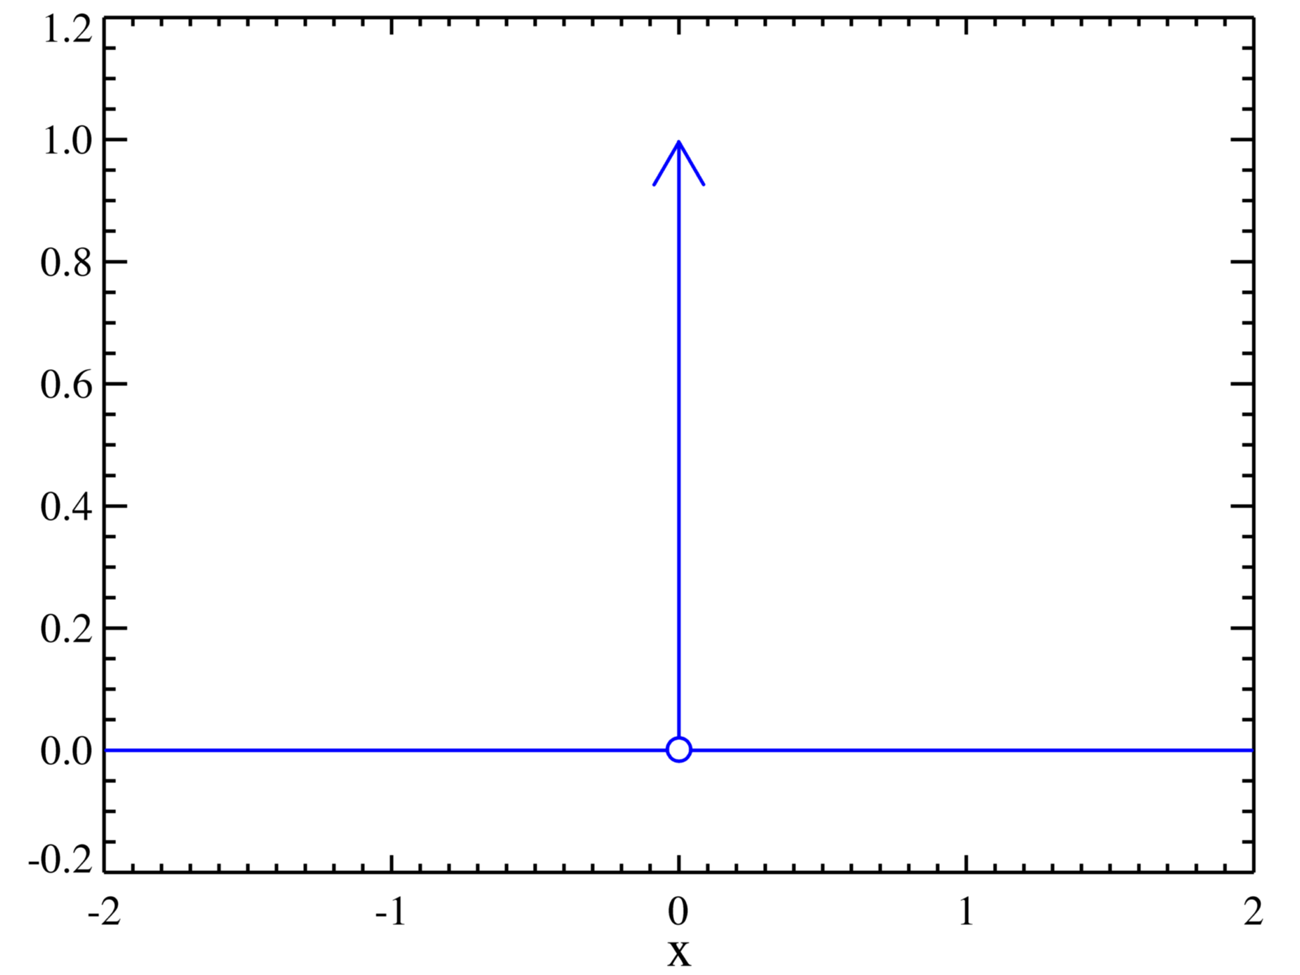
\includegraphics[scale = 0.15]{Dirac_distribution_PDF.png}
\end{figure}


\newpage 

Da un punto di vista misuristico, la Delta di Dirac non ci aiuta perchè rappresenta solo un modello matematico, 
che non ha riscontri nei circuiti e nei segnali reali. \newline 

D'altra parte, Shannon, nel suo teorema non menziona mai la Delta di Dirac, ma ci dice che dobbiamo prendere i valori istantanei della funzione f(t). \newline 

\newpage 

\section{Fase 1: Campionamento}
\footnote{Slide della prof | SDME 3.Conversione AD e Convertitori - Parte I | pag 15 - 17 \\  
Appunti | 2025-03-18 | pag 6}

Per adattare e applicare il campionamento nell'ambito delle misure, dobbiamo applicare il teorema di Shannon e applicarlo con segnali reali. \newline 

Campionare un segnale analogico g(t) significa, sotto l'aspetto operativo, 
individuare la successione dei valori $g(t_0 + nT_c)$ dove $t_0$ è un istante iniziale arbitrario, 
n è un intero e $T_c$ è la quantità costante chiamata periodo di campionamento, in particolari istanti, detti "istanti di campionamento", 
temporaneamente equi-spaziati. \newline 

Dalla successione dei valori individuata mediante il campionamento è possibile, secondo il teorema del campionamento, 
ricavare univocamente il segnale analogico g(t) se il segnale g(t) rispetta le seguenti proprietà: 

\begin{enumerate}
    \item g(t) deve avere banda limitata 
    \item il tempo che separa due successivi istanti di campionamento è minore di un valore critico stabilito dalle caratteristiche del segnale analogico 
    \item si acquisiscono 2x infiniti campioni
\end{enumerate}

Riguardo al primo punto, se si considera un segnale reale con infinite frequenze, 
è possibile applicare un filtraggio, ma bisogna valutare se le frequenze che il filtro toglie sono importanti per la nostra trattazione. \newline 

L'ultima condizione riguardo agli infiniti valori, è impossibile da mettere nella pratica. \newline 

\begin{tcolorbox}
    Regola aurea del mondo reale: è difficile o quasi impossibile avere infiniti valori
\end{tcolorbox}

Per campionare il segnale analogico g(t) senza perdere informazione, 
il periodo di campionamento $T_c$, cioè la distanza temporale fra due successivi campioni, deve essere: 

{
    \Large 
    \begin{equation}
        T_c < \frac{1}{2B}
    \end{equation}
}

dove B è la banda del segnale determinata dalla frequenza più alta che si trova nel suo spettro (lo si può notare dalla serie di Fourier del segnale). \newline 

Quindi, si può applicare il campionamento solo per segnali a banda limitata. \newline 

Definiamo la frequenza di campionamento $f_c$ l'inverso del tempo di campionamento $T_c$: 

{
    \Large 
    \begin{equation}
        f_c = \frac{1}{T_c}
    \end{equation}
}

La frequenza di campionamento $f_c$ deve essere:

{
    \Large 
    \begin{equation}
        f_c > f_N 
    \end{equation}
}

dove: 

{
    \Large 
    \begin{equation}
        f_N = 2B
    \end{equation}
}

$f_N$ prende il nome di frequenza di Nyquist. \newline 

La frequenza di Nyquist varierà in base alla banda del segnale in esame. \newline 

\newpage 

\subsection{Fase 1: Campionamento e aliasing (prima parte)}
\footnote{Slide della prof | SDME 3.Conversione AD e Convertitori - Parte I | pag 18 - 20 \\  
Appunti | 2025-03-18 | pag 6 - 7}

\begin{tcolorbox}
    Nota a lezione: aliasing è un termine latino, quindi si legge all'italiana
\end{tcolorbox}

Consideriamo un segnale sinusoidale nel tempo. \newline 

Se campioniamo a una frequenza di campionamento $f_c$: 

{
    \Large 
    \begin{equation}
        f_c = 8B
    \end{equation}
}

il campionamento individuerà i seguenti punti nel segnale: 

\begin{figure}[h]
    \centering
    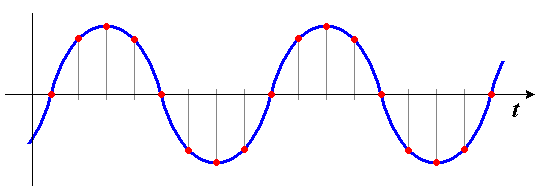
\includegraphics[scale = 0.6]{Frequenza di campionamento a 8B.png}
\end{figure}

Questa sinusoide passa per i punti (quelli che nella figura sono di colore rosso) individuati, quindi è univocamente determinata. \newline 

Considerando una frequenza di campionamento $f_c$ : 

{
    \Large 
    \begin{equation}
        f_c = 4B
    \end{equation}
}

il campionamento individuerà i seguenti punti nel segnale: 

\begin{figure}[h]
    \centering
    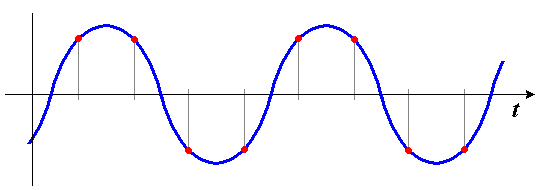
\includegraphics[scale = 0.6]{Frequenza di campionamento a 4B.png}
\end{figure}

Come il caso precedente della frequenza di campionamento a 8B, 
a questa frequenza di campionamento 
questa sinusoide passa per i punti (quelli che nella figura sono di colore rosso) individuati, quindi è univocamente determinata. \newline 

Se consideriamo la frequenza di campionamento $f_c$ esattamente: 

{
    \Large 
    \begin{equation}
        f_c = 2B
    \end{equation}
}

il campionamento può trovare questi due casi: 

\begin{figure}[h]
    \centering
    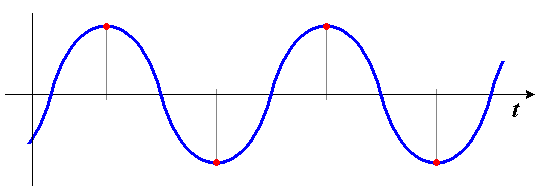
\includegraphics[scale = 0.6]{Frequenza di campionamento a 2B caso 1.png}
    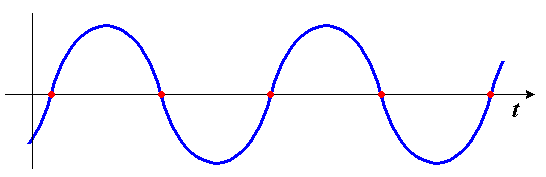
\includegraphics[scale = 0.6]{Frequenza di campionamento a 2B caso 2.png}
\end{figure}

\newpage 

Rispetto ai casi della frequenza di campionamento maggiore di 2B, 
in questo caso, possiamo trovare infinite funzioni che possono passare per i punti individuati: 
per questo motivo si dice che esiste un errore di alias. \newline 

Se campioniamo a frequenza esattamente uguale al doppio della banda, 
non siamo in grado di individuare univocamente la funzione che passa per quei punti. \newline 

Shannon, nel suo teorema del campionamento, aveva scritto che, per campionare, bisognare ricavare univocamente il segnale analogico. \newline 

In questo caso, non essendo univocamente identificata una funzione dopo il campionamento,  
troviamo infinite funzioni alla stessa frequenza, ma diversa ampiezza. \newline 

Considerando il caso peggiore, cioè campionando ad una frequenza di campionamento minore di 2B, ad esempio: 

{
    \Large 
    \begin{equation}
        f_c = 1.33B
    \end{equation}
}

il segnale campionato potrà essere:

\begin{figure}[h]
    \centering
    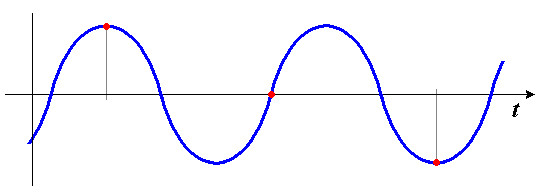
\includegraphics[scale = 0.6]{Frequenza di campionamento a 1,33B caso 1.png}
\end{figure}

Interpolando i punti: 

\begin{figure}[h]
    \centering
   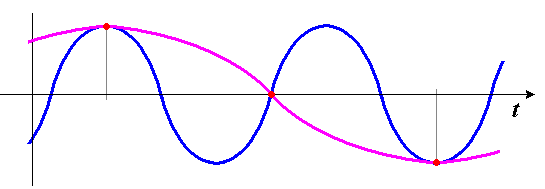
\includegraphics[scale = 0.6]{Frequenza di campionamento a 1,33B caso 2.png}
\end{figure}


Il segnale in viola è una possibile funzione che interpola i punti della funzione campionata, 
che è, come si nota dalla figura, un segnale sotto-campionato. \newline 

Dalle figure dei segnali sotto-campionati, si può formalizzare la seguente osservazione: 
se si riduce la frequenza di campionamento $f_c$ sotto al limite di Shannon, non si è più in grado di individuare univocamente 
la frequenza della funzione originale. \newline 

\newpage 

\section{Fase 1: Campionamento (seconda parte)}
\footnote{Slide della prof | SDME 3.Conversione AD e Convertitori - Parte I | pag 21 - 25 \\  
Appunti | 2025-03-18 | pag 7 - 8}

Considerando una frequenza di campionamento $f_c$ maggiore di quella di campionamento, 
si evita l'incongruenza di alias. \newline 

Se si riesce a rispettare questa condizione, 
NON si ha perdita di informazione nella fase di campionamento .\newline 

Considerando il segnale originale analogico, come in figura: 

\begin{figure}[h]
    \centering
    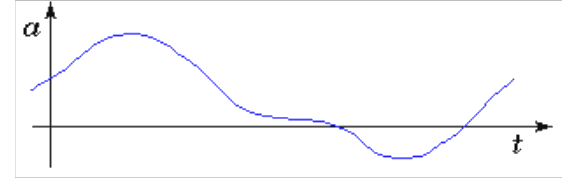
\includegraphics[scale = 0.6]{Esempio segnale analogico.png}
\end{figure}

il segnale è a tempo-continua e la vogliamo rendere a tempo-discreta. \newline 

Il primo passo è il seguente: 

\begin{figure}[h]
    \centering
    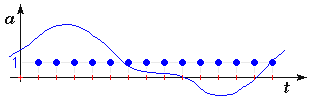
\includegraphics[scale = 1]{Segnale analogico moltiplicato per la funzione di campionamento.png}
\end{figure} 

Come si nota dalla figura, si moltiplica il segnale analogico per una funzione di campionamento di impulsi istantanei che ha l'andamento mostrato (quelli con il palloncino blu): 
essa è definita solo in corrispondenza degli istanti di campionamento e in quegli istanti il suo valore è unitario. \newline 

Questo funzione di campionamento NON è la Delta di Dirac, è un'altra funzione, perchè, nella Delta di Dirac l'ampiezza negli istanti $T_c$ tende a infinito. \newline 

Facendo il prodotto tra il "treno di impulsi unitario" e la funzione analogica da campionare, 
si ha la seguente funzione: 

\begin{figure}[h]
    \centering
    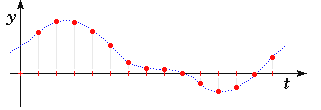
\includegraphics[scale = 1]{Segnale analogico campionato.png}
\end{figure} 

Come si nota dalla figura, tra un valore e l'altro (tra i due puntini rossi) la funzione non è definita in quegli istanti. \newline 

Sapendo dal corso di Segnali Determinati Aleatori che c'è una relazione tra tempo e frequenza tra due funzioni, 
se si fa una moltiplicazione nel tempo, allora in frequenza ci sarà una convoluzione tra i due segnali. \newline 

In frequenza il segnale analogico sarà:

\begin{figure}[h]
    \centering
    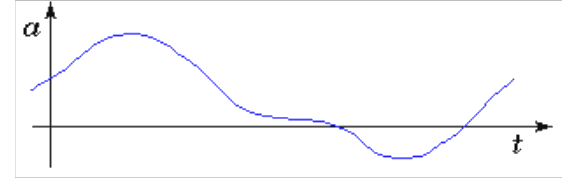
\includegraphics[scale = 0.6]{Esempio segnale analogico.png}
    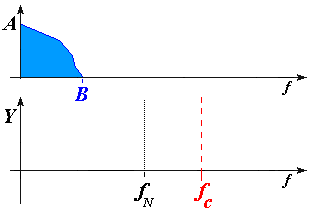
\includegraphics[scale = 0.6]{Banda del segnale analogico da campionare.png}
\end{figure}

\newpage 

Dallo spettro di frequenza (figura a destra), 
notiamo che la banda del segnale analogico B è minore della frequenza di campionamento $f_c$, 
e che la frequenza di campionamento $f_c$ è maggiore della frequenza di Nyquist $f_N$ relativo al segnale. \newline 

Se si considera il segnale di campionamento, avremo una riga in presenza di $f_c$: 

\begin{figure}[h]
    \centering
    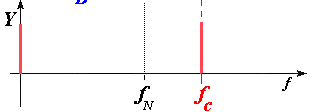
\includegraphics[scale = 1]{Segnale di campionamento in frequenza.png}
\end{figure} 

Facendo la circonvoluzione in frequenza tra il segnale analogico con banda B e il segnale degli impulsi unitari, 
avremo il seguente caso: 

\begin{figure}[h]
    \centering
    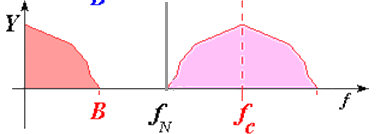
\includegraphics[scale = 1]{Convoluzione in frequenza tra generico segnale e treno di impulsi unitari.png}
\end{figure} 

\newpage 

Come avete studiato nel corso di Segnali Determinati Aleatori, 
la convoluzione genera delle repliche del segnale analogico originale per ogni $n f_c$ dove n è un numero intero. \newline 

Utilizzato un filtro come il seguente (denotato e tratteggiato di verde):

\begin{figure}[h]
    \centering
    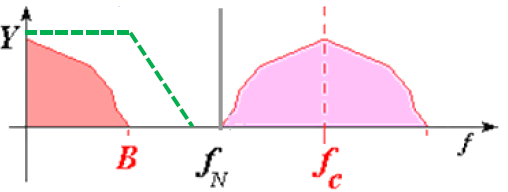
\includegraphics[scale = 0.6]{Convoluzione in frequenza tra generico segnale e treno di impulsi unitari con filtro realizzabile.png}
\end{figure} 

si può ricavare il segnale originale in banda base. \newline 

Non essendo un filtro ripido, è realmente realizzabile. \newline 

Se invece si dilata il tempo e si pone: 

{
    \Large 
    \begin{equation}
        f_c = f_N
    \end{equation}
}

e facendo la convoluzione, avremo il seguente caso: 


\begin{figure}[h]
    \centering
    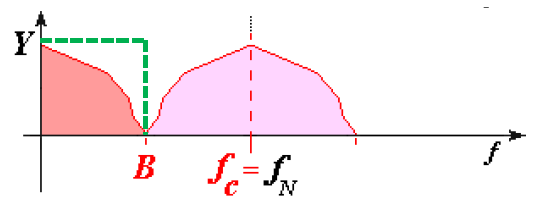
\includegraphics[scale = 0.6]{Convoluzione in frequenza tra generico segnale e treno di impulsi unitari con filtro NON realizzabile.png}
\end{figure} 

In questo caso, come indicato dalla linea tratteggiata verde, per recuperare il segnale campionato in banda base, 
il filtro è ideale e non fisicamente realizzabile. \newline 

Avremo un caso peggiore, quando: 

{
    \Large 
    \begin{equation}
        f_c < B
    \end{equation}
} 

e lo possiamo visualizzare nella seguente figura: 

\begin{figure}[h]
    \centering
    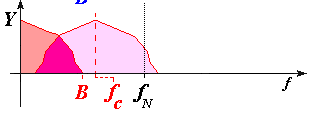
\includegraphics[scale = 1]{Convoluzione in frequenza tra generico segnale e treno di impulsi unitari al di sotto di B.png}
\end{figure} 

Come dimostrato da questi casi, 
il caso migliore per campionare un segnale senza avere aliasing è quello di: 

{
    \Large 
    \begin{equation}
        \begin{split}
            f_c &> 2B
            \\ 
            &\updownarrow
            \\ 
            T_c &< \frac{1}{2B}
        \end{split} 
    \end{equation}
}

cioè come possiamo visualizzare nel primo caso della convoluzione. \newline 

Più differenza c'è tra $f_c$ da $f_N$, tanto meno gravoso sarà il progetto del filtro passa-basso che bisognerà usare. \newline 

Una regola a "spanna" è quella di stare almeno a 20\% in più rispetto alla banda B per poter ricostruire il segnale 
con un LPF reale. \newline 

Campionando a una frequenza al di sotto di $f_N$, non avremo mai modo di recuperare il segnale originale perchè la convoluzione genera un segnale non lineare. \newline 

\newpage 

\section{Fase 2: Quantizzazione}
\footnote{Slide della prof | SDME 3.Conversione AD e Convertitori - Parte I | pag 26 - 30 \\  
Appunti | 2025-03-18 | pag 9 - 11}

Dalla conversione analogico-digitale, l'obbiettivo del campionamento, cioè la discretizzazione nel tempo del segnale, 
è quello di discretizzare anche le ampiezze del segnale analogico, quindi dobbiamo quantizzare il segnale campionato. \newline 

Quantizzare significa creare una divisione nelle ampiezze del segnale. \newline 

Per quantizzare il segnale campionato si deve, per prima cosa, fissare il campo di misura, 
cioè un intervallo di valori compreso fra un minimo ed un massimo: 
in altre parole dobbiamo individuare l'escursione massima del segnale. \newline 

Le scelte usuali per il campo di misura, se si considera come grandezza i volt, sono due: 

\begin{itemize}
    \item campo unipolare, cioè con estremi tra 0 ed $E_c$ volt 
    \item campo bipolare, cioè con estremi $-E_c$ e $+E_c$ volt (l'intervallo sarà simmetrico) 
\end{itemize}


Dopo aver stabilito il campo di misura, 
lo si suddivide in un numero arbitrario finito di intervalli contigui, cioè "uno dietro all'altro". \newline 

Gli intervalli possono essere di due tipi: 

\begin{itemize}
    \item intervalli di uguale ampiezza, si tratterà di quantizzazione uniforme 
    \item intervalli di ampiezza diversa, si tratterà di quantizzazione non uniforme
\end{itemize}

Consideriamo, per adesso, la quantizzazione uniforme. \newline 

Dopo aver stabilito il campo di misura e averlo diviso in N intervalli contigui, come in figura: 

\begin{figure}[h]
    \centering
    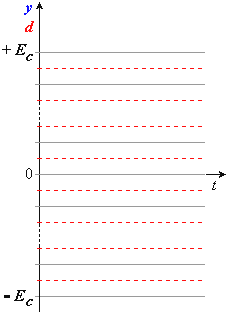
\includegraphics[scale = 1]{Divisione del campo bipolare.png}
\end{figure} 

bisogna individuare gli N valori del centro di ciascun intervallo in cui è stato suddiviso il campo di misura. \newline 

Nella figura, gli intervalli sono indicati con le linee grigie, 
invece il centro degli intervalli è indicato con le linee tratteggiate in rosso. \newline 

Considerando il caso in cui avremo un segnale quantizzato, 
avremo il seguente caso:

\begin{figure}[h]
    \centering
    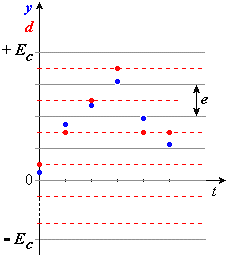
\includegraphics[scale = 1]{Campo bipolare con campioni da quantizzare.png}
\end{figure} 

\newpage 

Se consideriamo i puntini blu il segnale campionato, 
questo ultimo viene assegnato al valore centrale dell'intervallo 
più vicino, che è, appunto il puntino rosso. \newline 

A causa di questo "spostamento", nella quantizzazione, a differenza del campionamento, 
si ha una perdita dell'informazione originale. \newline 

Essendoci una perdita di informazione, si introduce una incertezza di quantizzazione. \newline 

Ogni valore quantizzato rappresenta l'ampiezza del valore campionato a meno di un valore $\pm \frac{e}{2}$. \newline 

Per ridurre l'entità di incertezza, dobbiamo ridurre il valore di e, cioè l'ampiezza degli intervalli di quantizzazione. \newline 

Ridurre il valore di e, non signfica modificare il campo, cioè modificare l'intervallo tra $[-E_c, + E_c]$, 
significa aumentare i livelli di quantizzazione. \newline 

La quantizzazione porta ad una alterazione del segnale: il valore originale del segnale nell'istante di campionamento 
viene alterato di una quantità che risulta, al massimo, pari alla semi-ampiezza dell'intervallo in cui esso cade. \newline 

Questa alterazione è chiamata incertezza di quantizzazione e, 
con campo bipolare e quantizzazione uniforme in N intervalli, vale: 

{
    \Large 
    \begin{equation}
        \begin{split}
            \Delta g 
            &= 
            \pm \left( \frac{2 E_c}{N}\right) \frac{1}{2}
            \\ 
            &= \pm \frac{2 E_c}{2N}
            \\
            &= \pm \frac{E_c}{N}
        \end{split}
    \end{equation}
}

Questo è un errore che possiamo calcolare prima di svolgere una misura. \newline 

La quantizzazione è una funzione univoca e non biunivoca: 

\begin{figure}[h]
    \centering
    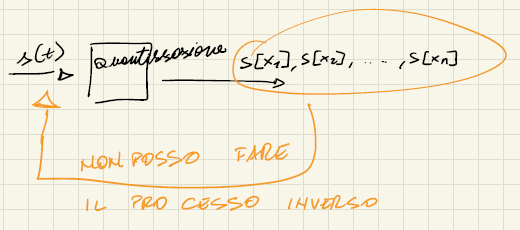
\includegraphics[scale = 0.8]{Quantizzazione funzione univoca.PNG}
\end{figure} 

\newpage

Essendoci un errore, la quantizzazione distorce il segnale originale: l'obbiettivo è rendere la distorsione la più piccola possibile. \newline 

Dalla formula di $\Delta g$, a parità di campo di misura, N è il parametro che definisce l'incertezza di quantizzazione. \newline 

Inoltre N influenza anche la codifica: ogni intervallo dovrà essere dotato di codifica univoca. \newline 

L'aumento dei livelli di quantizzazione significa anche avere maggiori bit, 
che serviranno per la codifica del segnale. \newline 

\newpage 

\subsection{Fase 2: Quantizzazione non silenziata}
\footnote{Slide della prof | SDME 3.Conversione AD e Convertitori - Parte I | pag 31 - 32 \\  
Appunti | 2025-03-18 | pag 11 | 2025-03-19 | pag 2}

Campionando un segnale nullo a cui è sovrapposto un rumore anche minimo, si avrebbero valori quantizzati non nulli e molto diversi l'uno dall'altro. \newline 

Come si nota dalle seguenti figure: 

\begin{figure}[h]
    \centering
    \includegraphics[scale = 0.45]{Rumore dopo che si è quantizzato in una quantizzazione non silenziata.png}
\end{figure} 

il rumore viene esaltato e sembra venire meno la capacità di reiezione al rumore dei segnali digitali. \newline 

\newpage 

\subsection{Fase 2: Quantizzazione silenziata}
\footnote{Slide della prof | SDME 3.Conversione AD e Convertitori - Parte I | pag 33 - 34 \\  
Appunti | 2025-03-19 | pag 2}

Per evitare l'amplificazione del rumore, si può applicare la quantizzazione silenziata dove esiste un intervallo "centrato" sul valore nullo, come si vede in figura: 

\begin{figure}[h]
    \centering
    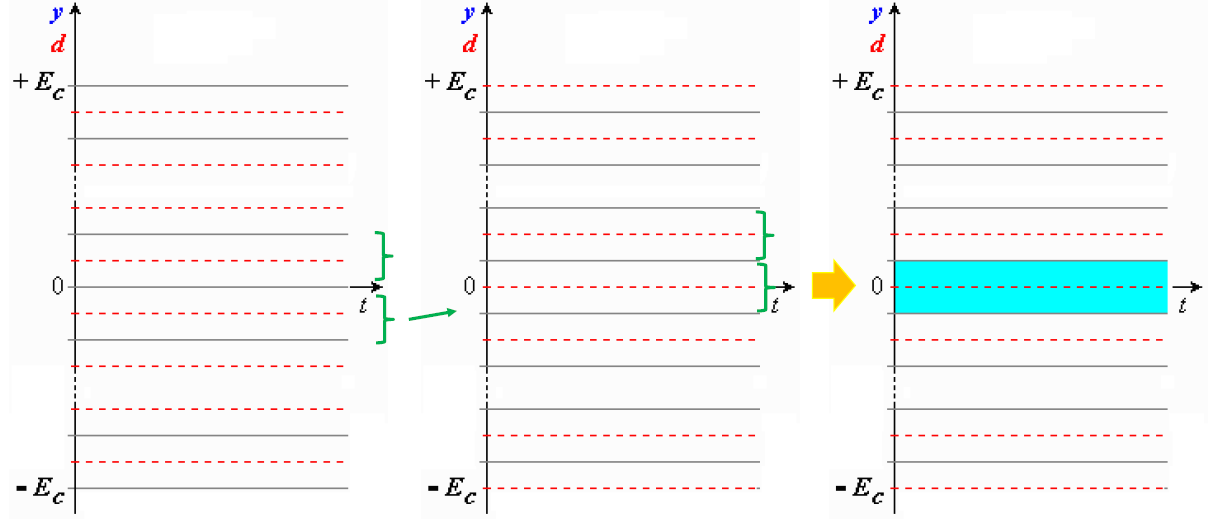
\includegraphics[scale = 0.45]{Da quantizzazione non silenziata a quantizzazione silenziata.png}
\end{figure} 

Grazie a questa scelta, lo zero volt è un livello di quantizzazione e quindi 
il rumore, che generalmente cade nell'intervallo "colorato in blu celestino", viene centrato a zero. \newline 

Grazie alla quantizzazione silenziata, si avrà una reiezione al disturbo perchè il rumore deve avere un'intensità non trascurabile per manifestarsi sul segnale. \newline 

A differenza della quantizzazione non silenziata, se esiste un disturbo con densità trascurabile si avrà il seguente caso: 

\begin{figure}[h]
    \centering
    \includegraphics[scale = 0.45]{Rumore dopo che si è quantizzato in una quantizzazione silenziata.PNG}
\end{figure} 

Inoltre, quando i valori del segnale campionato arrivano ai livelli di campo, 
cioè $-E_c$ e $+E_c$, non vengono neanche elaborati e/o presi in considerazione dal quantizzatore. \newline 

\newpage 

\section{Fase 2: Quantizzazione - conclusioni}
\footnote{Slide della prof | SDME 3.Conversione AD e Convertitori - Parte I | pag 35 \\  
Appunti | 2025-03-19 | pag 2}

Al termine della fase 2 della conversione da analogico a digitale, quindi alla fine della quantizzazione, 
si ha un segnale discretizzato sia nei tempi che nelle ampiezze perchè può assumere solo un numero limitato di valori, quelli individuati dagli intervalli di quantizzazione. \newline 

Quindi, dal segnale analogico, si è passati al segnale campionato, al segnale quantizzato: 

\begin{figure}[h]
    \centering
    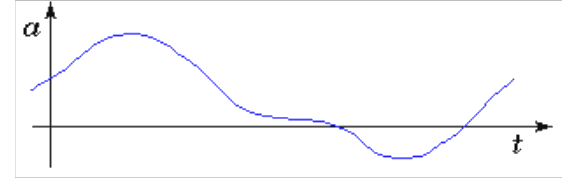
\includegraphics[scale = 0.45]{Esempio segnale analogico.png} 
    \\
    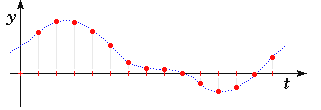
\includegraphics[scale = 0.8]{Segnale analogico campionato.png}
    \\
    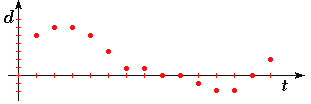
\includegraphics[scale = 0.8]{Segnale quantizzato.png}
\end{figure} 

Per concludere, la scelta dell'ADC si baserà su: 

\begin{itemize}
    \item frequenza di campionamento $f_c$ 
    \item risoluzione
\end{itemize}

\newpage 